%%*************************************************************************
%% Legal Notice:
%% This code is offered as-is without any warranty either expressed or
%% implied; without even the implied warranty of MERCHANTABILITY or
%% FITNESS FOR A PARTICULAR PURPOSE! 
%% User assumes all risk.
%% In no event shall the IEEE or any contributor to this code be liable for
%% any damages or losses, including, but not limited to, incidental,
%% consequential, or any other damages, resulting from the use or misuse
%% of any information contained here.
%%
%% All comments are the opinions of their respective authors and are not
%% necessarily endorsed by the IEEE.
%%
%% This work is distributed under the LaTeX Project Public License (LPPL)
%% ( http://www.latex-project.org/ ) version 1.3, and may be freely used,
%% distributed and modified. A copy of the LPPL, version 1.3, is included
%% in the base LaTeX documentation of all distributions of LaTeX released
%% 2003/12/01 or later.
%% Retain all contribution notices and credits.
%% ** Modified files should be clearly indicated as such, including  **
%% ** renaming them and changing author support contact information. **
%%*************************************************************************


% *** Authors should verify (and, if needed, correct) their LaTeX system  ***
% *** with the testflow diagnostic prior to trusting their LaTeX platform ***
% *** with production work. The IEEE's font choices and paper sizes can   ***
% *** trigger bugs that do not appear when using other class files.       ***                          ***
% The testflow support page is at:
% http://www.michaelshell.org/tex/testflow/


% Please refer to your journal's instructions for other
% options that should be set.
\documentclass[conference,onecolumn,10pt]{IEEEtran}
\usepackage[section]{placeins}
\usepackage{enumerate}
\usepackage{makecell} 
\usepackage{graphicx}
\usepackage{url}
\usepackage[spanish]{babel}
\usepackage[utf8]{inputenc}
\usepackage[backend=biber, style=numeric]{biblatex}
\addbibresource{Presentacion.bib}

% If IEEEtran.cls has not been installed into the LaTeX system files,
% manually specify the path to it like:
% \documentclass[journal]{../sty/IEEEtran}
\author{\IEEEauthorblockN{Alberto de Jesús Sánchez López}
\IEEEauthorblockA{Universidad Veracruzana\\
Ingeniería de Software\\
Veracruz, México\\
Email: zs15011648@estudiantes.edu.mx}
\and
\IEEEauthorblockN{M.C.C. María Angélica Cerdán}
\IEEEauthorblockA{Universidad Veracruzana\\
Veracruz, México\\
}
\and
\IEEEauthorblockN{Dr. Jorge Octavio Ocharán Hernández}
\IEEEauthorblockA{Universidad Veracruzana\\
Veracruz, México\\}}

\hyphenation{op-tical net-works semi-conduc-tor}

\begin{document}

% paper title
% Titles are generally capitalized except for words such as a, an, and, as,
% at, but, by, for, in, nor, of, on, or, the, to and up, which are usually
% not capitalized unless they are the first or last word of the title.
% Linebreaks \\ can be used within to get better formatting as desired.
% Do not put math or special symbols in the title.
\title{Revisión de la literatura sobre las actividades de \\ requisitos para Software como Servicio}
% author names and IEEE memberships
% note positions of commas and nonbreaking spaces ( ~ ) LaTeX will not break
% a structure at a ~ so this keeps an author's name from being broken across
% two lines.
% use \thanks{} to gain access to the first footnote area
% a separate \thanks must be used for each paragraph as LaTeX2e's \thanks
% was not built to handle multiple paragraphs

% The paper headers

\markboth{Universidad Veracruzana - Ingeniería de Software - Proyecto Guiado}%
{Shell \MakeLowercase{\textit{et al.}}: Bare Demo of IEEEtran.cls for IEEE Journals}

% If you want to put a publisher's ID mark on the page you can do it like
% this:
%\IEEEpubid{0000--0000/00\$00.00~\copyright~2015 IEEE}
% Remember, if you use this you must call \IEEEpubidadjcol in the second
% column for its text to clear the IEEEpubid mark.



% use for special paper notices
%\IEEEspecialpapernotice{(Invited Paper)}

% make the title area
\maketitle

% As a general rule, do not put math, special symbols or citations
% in the abstract or keywords.
\begin{abstract}
\end{abstract}

% Note that keywords are not normally used for peerreview papers.
\begin{IEEEkeywords}
\end{IEEEkeywords}

\section{Introducción}
% The very first letter is a 2 line initial drop letter followed
% by the rest of the first word in caps.
% 
% form to use if the first word consists of a single letter:
% \IEEEPARstart{A}{demo} file is ....
% 
% form to use if you need the single drop letter followed by
% normal text (unknown if ever used by the IEEE):
% \IEEEPARstart{A}{}demo file is ....
% 
% Some journals put the first two words in caps:
% \IEEEPARstart{T}{his demo} file is ....
% 
% Here we have the typical use of a "T" for an initial drop letter
% and "HIS" in caps to complete the first word.
\IEEEPARstart{T}{his} demo file is intended to serve as a ``starter file''
for IEEE journal papers produced under \LaTeX\ using
IEEEtran.cls version 1.8b and later.
% You must have at least 2 lines in the paragraph with the drop letter
% (should never be an issue)

\section{Trabajos relacionados}
\newpage

\section{Método de investigación}
\subsection{Preguntas de investigación}

El objetivo de la Revisión Sistemática de la Literatura es encontrar el estado del arte del las actividades de requisitos para un \emph{software} como servicio. 

\begin{enumerate}[P 1.-]
  \item\emph{¿Qué técnicas de elicitación se han utilizado para la identificación de requisitos de Software como Servicio?}
  \begin{enumerate}[(a)]
  \item \emph{¿Qué retos se presentan en la elicitación?}
  \end{enumerate}
  Motivación: Señalar el conjunto de técnicas utilizadas para llevar a cabo un proceso de elicitación de requisitos para un software como servicio e identificar los retos encontrados en el proceso de elicitación. 
  
  \item\emph{¿Qué técnicas de análisis se han utilizado para la definición de requisitos de Software como Servicio?}\\
  Motivación: Identificar las actividades realizadas para llevar a cabo el proceso de análisis, clasificación y definición de un conjunto de requisitos para un software como servicio.

  \item\emph{¿Qué actividades se han utilizado para llevar a cabo la validación de los requisitos de un Software como Servicio?}\\
  Motivación: Identificar las técnicas que utilizadas para definir un proceso de validación de requisitos para un software como servicio.

  \item\emph{¿Qué temas abiertos se identifican en la literatura reciente en el desarrollo de Software como Servicio?}
  \begin{enumerate}[(a)]
  \item \emph{¿Qué temas abiertos existen relacionados a las actividades llevadas a cabo en la gestión de requisitos de un software como servicio?}
  \end{enumerate}
  Motivación: Identificar los temas abiertos sugeridos en la literatura relacionada a las actividades de elicitación, análisis, validación y gestión de cambios 
 para requisitos de un software como servicio.
\end{enumerate}

\subsection{Proceso de búsqueda}

\begin{table}[ht]
        \caption{Términos de búsqueda} 
        \centering 
        \scalebox{1.3}{
        \begin{tabular}{c c}
                \hline
                Concepto & Término de búsqueda\\ [0.5ex] 
                \hline
                Requisitos             & \makecell{Requirements Engineering \\
                                                   Collaborative Requirements} \\
                \hline 
                Software como servicio & \makecell{Software as a Service \\
                                                   SaaS \\
                                                   Cloud Computing }\\ [1ex]
                \hline 
        \end{tabular}}
        \label{table:tablaterminos}
\end{table}

\subsection{Proceso de selección}
\subsection{Estrategia de extracción de datos}
\subsection{Método de síntesis de datos}
\newpage

\section{Conducción}
\newpage


\section{Resultados}
Llevar a cabo el proceso de extracción, permitió realizar un análisis 
\begin{figure}[!htb]
   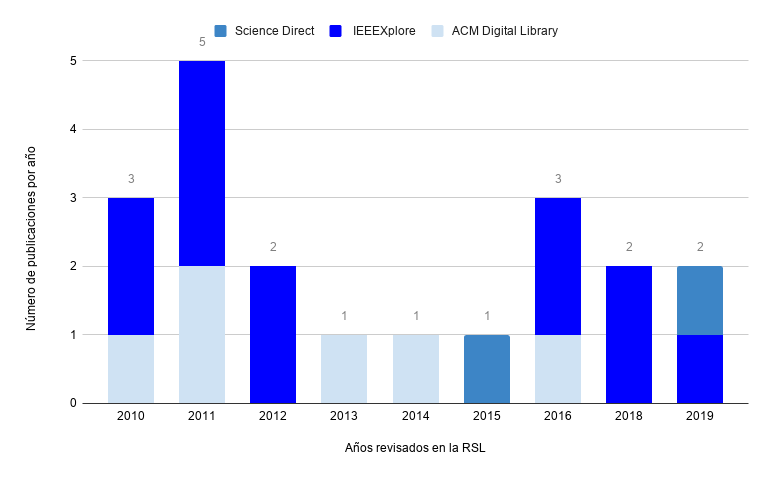
\includegraphics[width=\linewidth]{chart.png}
   \caption{Estudios primarios por año de publicación.}
   \label{fig:estudiostotales}
\end{figure}

Llevar a cabo el proceso de extracción, permitió realizar un análisis 

\begin{table}[ht]
\centering
        \scalebox{1.2}{
        \begin{tabular}{c c c c}
                \hline
                ID & Autor(es) & Año de publicación & Referencia \\ [0.5ex] % inserts table
                %heading
                \hline
                EF-1 & Xin Zhou, Li Yi, Ying Liu & 2010 & \cite{EF-1} \\
                \hline
                EF-2 & \makecell{Rafael Chanin, Leandro Pompermaier, Afonso Sales, Rafael Prikladnicki} & 2019 & \cite{EF-2} \\
                \hline 
                EF-3 & Pedro Cecilio Lopes, Alberto Rodrigues da Silva & 2018 & \cite{EF-3} \\
                \hline 
                EF-4 & Nupul Kukreja & 2012 & \cite{EF-4} \\
                \hline 
                EF-5 & Wantana Singhto, Nuttaporn Phakdee & 2011 & \cite{EF-5} \\
                \hline 
                EF-6 & Claudia Litvak, Leandro Antonelli, Gustavo Rossi, Nora Gigante & 2018 & \cite{EF-6} \\
                \hline 
                EF-7 & Ince T Wangsa, Lorna Uden, Stella F Mills  & 2011 & \cite{EF-7} \\
                \hline 
                EF-8 & Diogo Duarte, Carla Farinha, Miguel Mira da Silva, Alberto Rodrigues da Silva  & 2012 & \cite{EF-8} \\
                \hline 
                EF-9 & Sergio F. Ochoa, Alcides Quispe, Andrés Vergara, José A. Pino & 2010 & \cite{EF-9} \\
                \hline 
                EF-10 & Wantana Singhto, Nuttaporn Phakdee & 2016 & \cite{EF-10} \\
                \hline
                EF-11 & Anum Tariq, Shoab Ahmed Khan, Sundas Iftikhar & 2014 & \cite{EF-11} \\
                \hline 
                EF-12 & Maalem Derdour Sourour, Nacereddine Zarour & 2011 & \cite{EF-12} \\
                \hline 
                EF-13 & Amro Najjar, Christophe Gravier, Xavier Serpaggi, Olivier Boissier & 2016 & \cite{EF-13} \\
                \hline 
                EF-14 & Stefan T. Ruehl, Holger Wache, Stephan A. W. Verclas & 2013 & \cite{EF-14} \\
                \hline 
                EF-15 & Mohamed A Abd Elmoniem, Eman S Nasr, Mervat H Gheith & 2016 & \cite{EF-15} \\
                \hline 
                EF-16 & Jaekeun Shim, Jongdae  Han, Jindae  Kim, Byeongjeong  Lee, Jaewon  Oh, Chisu  Wu  & 2011 & \cite{EF-16} \\
                \hline 
                EF-17 & Shehnila Zardari, Rami  Bahsoon & 2011 & \cite{EF-17} \\
                \hline 
                EF-18 & Soonhwa Lee-Klenz, Pedro R Falcone Sampaio, Trevor A Wood-Harper  & 2010 & \cite{EF-18} \\
                \hline 
                EF-19 & Jorge Melegatia, Alfredo Goldman, Fabio Kon, Xiaofeng Wang & 2019 & \cite{EF-19} \\
                \hline 
                EF-20 & Ivan Prakasa, Osamu Shigo & 2015 & \cite{EF-20} \\
                \hline 
        \end{tabular}}
        \label{table:tablaterminos}
\end{table}

\section{Amenazas a la validez}

\section{Discusión}

\section{Conclusión}
The conclusion goes here.





% if have a single appendix:
%\appendix[Proof of the Zonklar Equations]
% or
%\appendix  % for no appendix heading
% do not use \section anymore after \appendix, only \section*
% is possibly needed

% use appendices with more than one appendix
% then use \section to start each appendix
% you must declare a \section before using any
% \subsection or using \label (\appendices by itself
% starts a section numbered zero.)

\appendices
\section{Proof of the First Zonklar Equation}
Appendix one text goes here.

% you can choose not to have a title for an appendix
% if you want by leaving the argument blank
\section{}
Appendix two text goes here.

% trigger a \newpage just before the given reference
% number - used to balance the columns on the last page
% adjust value as needed - may need to be readjusted if
% the document is modified later
%\IEEEtriggeratref{8}
% The "triggered" command can be changed if desired:
%\IEEEtriggercmd{\enlargethispage{-5in}}

% references section

% can use a bibliography generated by BibTeX as a .bbl file
% BibTeX documentation can be easily obtained at:
% http://mirror.ctan.org/biblio/bibtex/contrib/doc/
% The IEEEtran BibTeX style support page is at:
% http://www.michaelshell.org/tex/ieeetran/bibtex/
%\bibliographystyle{IEEEtran}
% argument is your BibTeX string definitions and bibliography database(s)
%\bibliography{IEEEabrv,../bib/paper}
%
% <OR> manually copy in the resultant .bbl file
% set second argument of \begin to the number of references
% (used to reserve space for the reference number labels box)
\printbibliography


% biography section
% 
% If you have an EPS/PDF photo (graphicx package needed) extra braces are
% needed around the contents of the optional argument to biography to prevent
% the LaTeX parser from getting confused when it sees the complicated
% \includegraphics command within an optional argument. (You could create
% your own custom macro containing the \includegraphics command to make things
% simpler here.)
%\begin{IEEEbiography}[{\includegraphics[width=1in,height=1.25in,clip,keepaspectratio]{mshell}}]{Michael Shell}
% or if you just want to reserve a space for a photo:

% You can push biographies down or up by placing
% a \vfill before or after them. The appropriate
% use of \vfill depends on what kind of text is
% on the last page and whether or not the columns
% are being equalized.
\end{document}
